\documentclass{article}
\usepackage{graphicx}
\usepackage[left=1.25in,right=1.25in]{geometry}
\usepackage{color}
\usepackage{amsmath}
\definecolor{Yellow}{rgb}{1,1,0}
\newcommand{\mat}[1]{\begin{bmatrix}#1\end{bmatrix}}
\newcommand{\edit}[1]{\colorbox{Yellow}{#1}}
%\newcommand{\edit}[1]{}
\newcommand{\dee}[2]{\frac{\partial{#1}}{\partial{#2}}}
\begin{document}
  \section*{Problem 1}
  \textit{Consider training a single perceptron with the perceptron
    activation rule.  Assume that an image is a $3\times 3$ array of
    pixels, with each pixel being on or off. For each of the following
    features, either present a perceptron that recognizes the feature
    or prove none exists.}

  We assume that an on pixel gives an input of 1 to the perceptron,
  and that an off pixel gives 0.

  Lemma: for any perceptron and any particular pixel, there cannot be
  a situation in which turning the pixel from off to on changes the
  output from negative to positive, and also another situation in
  which it does the reverse, since the first requires that its weight
  be positive, while the second requires that its weight be negative.

  \begin{enumerate}
  \item \textbf{bright or dark} --- At least 75\% of the pixels are
    on, or at least 75\% of the pixels are off.

    No --- The input condition requires that 0, 1, 2, 7, 8, or 9
    pixels are on. Consider one input with exactly 6 pixels on, not
    including the top right pixel, and another one with exactly 2 on,
    not including that pixel. Turning on the top right pixel proves
    impossibility, by the lemma.

  \item \textbf{top-bright} --- a larger fraction of pixels is on in
    the top row than in the bottom two rows.

    Yes --- each pixel in the top row has a weight of 2, and all other
    pixels have a weight of $-1$. The threshold is 0.

    %% we present one that exists.  Let $a_1,a_2,a_3$ be the first row
    %% and $a_4,\ldots,a_9$ be the bottom two rows. Our perceptron
    %% classifier can be as follows: letting $a_i=0$ denote off and
    %% $a_i=1$ denote on,
    %% $$P(a_1,\ldots,a_9)=2(a_1+a_2+a_3)-(a_4+\ldots+a_9)$$
    %% is positive if a larger fraction of pixels are on in the top row than
    %% in the bottom two rows, and nonpositive otherwise. 

  \item \textbf{connected}

    No --- Consider the following inputs.

    \[\mat{1&0&0\\0&0&0\\0&0&0}\qquad\mat{1&0&1\\0&0&0\\0&0&0}\qquad\mat{0&1&0\\0&0&1\\0&0&0}\qquad\mat{0&1&1\\0&0&1\\0&0&0}\]

    Considering the first two, we see that turning on the top right
    pixel can change the state from connected to unconnected; but in
    the other two, turning it on does the reverse. Impossible by the
    lemma.
  \end{enumerate}

  \section*{Problem 2}
  \textit{Consider four different possible learning algorithms for the
    digits classification problem and argue for or against each of
    them given that decision trees can be continuous:}
  \begin{itemize}
  \item decision trees --- These tend to be best when a small number
    of attributes are particularly important. For this problem,
    individual inputs matter much less than the relationship between
    them; decision trees would have a hard time capturing that well.
  \item boosted decision stumps --- similar to above; even though they
    perform well for identifying cancer characteristics, a weighted
    average of several splits would not be useful for identifying
    digits because of the importance of specific interactions between
    groups of inputs.
  \item perceptrons --- linear separation is very limited. They can't
    tell connectedness or separation. In order for it to work we would
    need to feed it higher level features ahead of time.
  \item multi-layer feed-forward neural networks --- this appears most
    promising.  It is good when many features have to be taken into
    account simultaneously but independently, which applies to our
    problem. It also can make complex decision boundaries to arbitrary
    precision given enough nodes in a single hidden layer. One
    downside is that if we have a working neural network, it would be
    difficult to look into it to figure out exactly how different
    factors work together, as we would be able to in decision trees.
  \end{itemize}

  \section*{Problem 3}
  \textit{Do you really think you need to answer this example
    question in your writeup?}

  No.

  \begin{enumerate}

    \setcounter{enumi}1
  \item \textbf{XOR} \textit{Include a picture of the network
    generated. Explain how the combination of weights emulates the
    logical operations needed to express XOR.}

    \begin{center}
      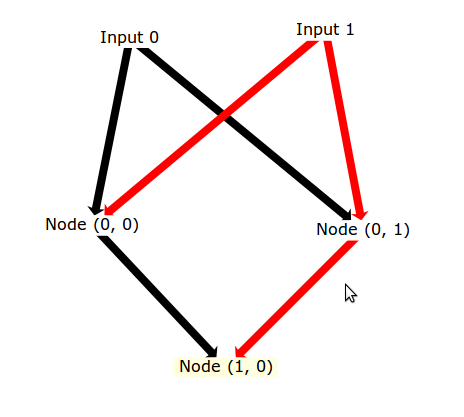
\includegraphics[scale=.4]{xor_net.png}
    \end{center}

    Weights resulting from a run (hidden nodes in the first line,
    output node in the second):

    \[(2.324, 2.727, -2.764)\qquad(-3.896, 3.412, -3.563)\]
    \[(2.406, -5.169, 5.186)\]

    In each tuple, the first value represents the bias $w_0$, and the
    remaining values are the weights of its variable inputs. The left
    node in the hidden layer corresponds to $(x_1\wedge\lnot x_2)$,
    while the right one corresponds to $(x_1\vee\lnot x_2)$, or
    $\lnot(\lnot x_1\wedge x_2)$.

    The output node corresponds to $(i_1\vee\lnot i_2)$, where $i_1$
    and $i_2$ are its inputs. Thus the whole net represents
    $((x_1\wedge\lnot x_2)\vee(\lnot x_1\wedge x_2))$, which is
    exactly $(x_1\oplus x_2)$.

    Plots of the activation levels of the two hidden nodes and the
    output node (as a function of the two inputs) have been included
    below.

    \begin{center}
      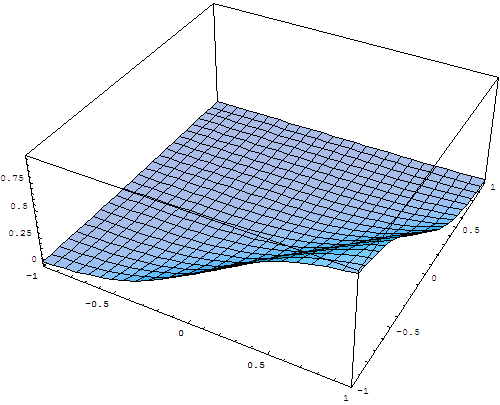
\includegraphics[scale=.35]{hidden1.png}
      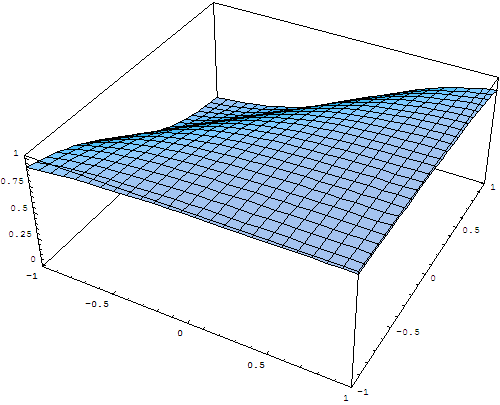
\includegraphics[scale=.35]{hidden2.png}
      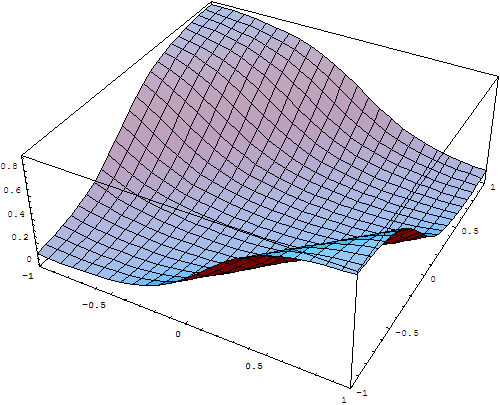
\includegraphics[scale=.35]{output.png}
    \end{center}

    \textit{What are some reasons the networks could intermittently
      fail to learn XOR?  What parameters can you tune to alleviate
      this type of problem?}

    The weights for one incorrect output net are as follows:

    \[(-7.117, 4.143, -4.186)\qquad(-6.529, 3.440, -3.485)\]
    \[(-.571, 2.693, 1.010)\]

    Now both of the hidden nodes are sort of computing $x_1\wedge\lnot
    x_2$. (I say ``sort of'' because their activation levels are only
    about .5 for input $(1,-1)$.) The output activation level is .8916
    for input $(1,-1)$ and about .361 for the other three.

    TODO why does this actually happen?

    If the training data were not sufficiently randomized, i.e.  if
    the network was trained on the same data repeatedly, AND if it had
    too high of a learning rate, then it could set its weights too
    strongly to classify the data it had seen repeatedly, and then not
    converge when it is trained on the rest of the data. In other
    words, it's possible that the neural network gets stuck in a local
    (error) minimum.
      
    We could reduce learning rate to make this less likely. 

    \edit{Does increasing epochs help? The interface is confusing.}

  \item \textbf{Experimental Analysis}
    \begin{enumerate}
    \item \textit{Provide the learning rate you used. How did you
      select this rate?}

      We think the optimal rate is about $.1$. We ran a great many
      trials, with varying ranges of learning rates. Included below
      are plots of performance on the test set after 40 rounds. (Each
      data point represents only one run, so the statistical
      significance is maybe not that good, but the trends seem to be
      visible.) Our thanks go to the NICE and Science Center basement
      machines.

      % TODO make these images

      With a step of .1 (learning rate ranging from .1 to 50):

      \begin{center}
        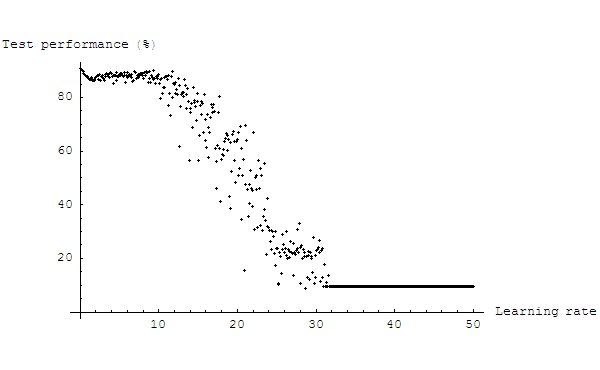
\includegraphics[scale=.5]{plot_test_1.png}
      \end{center}

      Clearly, the rate should not be more than 10. We continue to
      zoom in on what appears to be the best peak, way down at the
      left end of the graph.

      With a step of .01 (range .01 to 3):

      \begin{center}
        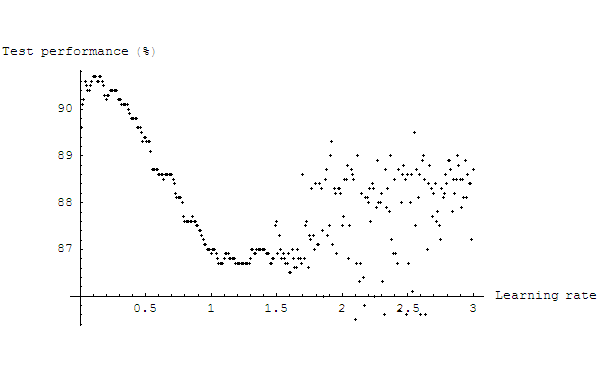
\includegraphics[scale=.5]{plot_test_01.png}
      \end{center}

      Still way at the left end.

      With a step of .001 (range .001 to 1):

      \begin{center}
        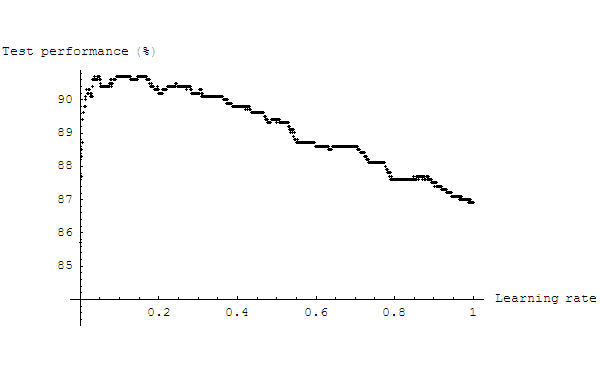
\includegraphics[scale=.5]{plot_test_001.png}
      \end{center}

      With a step of .0001 (range .0001 to .2):

      \begin{center}
        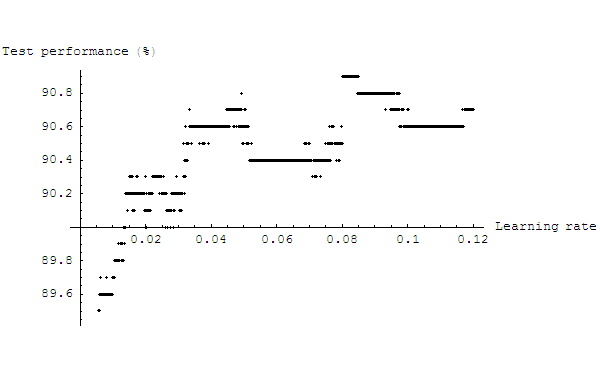
\includegraphics[scale=.5]{plot_test_0001.png}
      \end{center}

      So the differences between the different rates are pretty small
      at this point, but it looks like it's safe to say that something
      around .1 is best.

    \item \textit{For this learning rate, chart the training set and
      validation error against the number of epochs from 1 to 100.}

      \begin{center}
        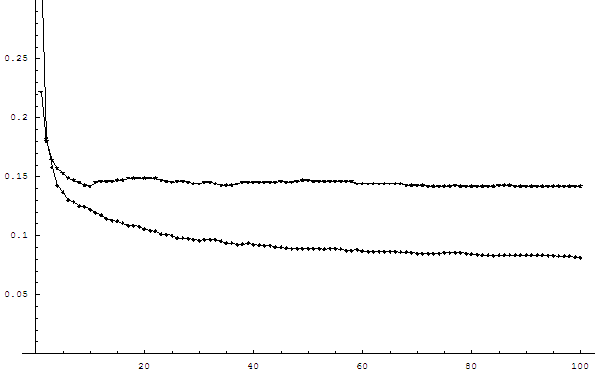
\includegraphics[scale=.4]{100_rounds.png}
      \end{center}

      The bottom line is the training set error; the top is validation
      set error.

      \begin{enumerate}
      \item \textit{Are we in danger of overfitting by training for
        too many epochs?}

        It doesn't really look like it; the validation set performance
        hardly goes down (and actually looks like it might be going
        up) as the number of rounds increases.

      \item \textit{What is a good number of epochs to train for?}

        At around 10 epochs, it looks like the validation performance
        has basically reached its stable value. and that's the
        smallest number of epochs to do so.

      \item \textit{Why is it important that we use a validation set
        (rather than the actual test set) to tune the number of
        epochs?}

        If we use the test set to tune the number of epochs, the
        tuning may overfit to the testing data, resulting in better
        reported performance. The point of the test set is that it
        doesn't affect the parameters of the net at all, so that it
        can provide an accurate measure of its performance.

      \end{enumerate}
    \item \textit{What is the training, validation, and test}
      performance \textit{of the network trained with your chosen
        learning rate and number of epochs?}

      After the last epoch, the training performance is 91.85\%, the
      validation performance is 85.80\%, and the test performance is
      90.50\%.
    \end{enumerate}

  \item \textbf{Model Selection}
    \begin{enumerate}
    \item \textit{Experiment with the distributed and binary encoding
      for both 15 and 30 hidden layers. Which encoding performs
      better? Is this in line with what we know about encodings? Use
      the better encoding for the rest of this problem.}

      We believe that the distributed encoding should do better. 
      This is because the binary encoding does not encode in a way
      that makes sense; there is no property of the (images of the)
      digits that links all odd digits together while they all share
      a 1 in the least significant spot in a binary encoding, for 
      example. 

    \item \textit{Provide the learning rates you used for training 15
      and 30 hidden units.}

      \setcounter{enumii}3

    \item \textit{In three sentences or less, explain your stopping
      condition.}

    \item \textit{For both 15 and hidden units, use your algorithm to
      determine when to stop.  Graph training data and validation set
      performance against the number of epochs you trained for.}

    \item \textit{How many epochs did you use for 15 hidden units?
      30?}

    \item \textit{What is the test performance for 15 and 30 hidden
      units? Does this agree with the validation set performance you
      observed? Which network structure (15, 30, 0 hidden units) would
      you choose based on these experiments?}

    \end{enumerate}


  \end{enumerate}

  \section*{Problem 4}
  \textit{Back-propagation for neural networks performs gradient
    descent on the error function}
  \[E(w)=\frac{1}{2}\sum_{d=1}^n\sum_{k=1}^K(y_{dk}-a_{dk})^2\]
  \textit{when there are $n$ examples $(x_d,y_d)$ and $K$ output units
    so that $y_d\in [0,1]^K$. (Note we index examples by $d$.)}

  \textit{Consider an alternative error function}
  \[F(W)=\frac12\sum_{d=1}^n\sum_{k=1}^K(y_{dk}-a_{dk})^2+\gamma\sum_{j\in V}\sum_{i\in\text{Parents}(j)}w_{ji}^2\]
  \textit{where the sum in the latter term is taken over all pairs of
    units $i,j$ such that there is an edge from $i$ to $j$.}

  \begin{enumerate}
  \item \textit{Explain why you might want to use the error function
    $F$. What problem is it trying to address, and how does it address
    it?}

    The error function $F$ takes into account the sum of squares of weights
    in the network. Using such an error function will try to bound the
    weights of a network, thus preventing a case in which normal gradient
    descent ends up increasing (or decreasing) certain weights exceedingly far
    in the same direction, which can pose a problem as it makes it 
    slower to adjust a weight back if it is incorrect, and also because it pushes
    the activation of a node too far along the outsides of the sigmoid
    function to make much of a difference, so that too high of a weight
    from one input node decreases a neuron's sensitivity. 
    \edit{????....}

  \item \textit{Use gradient descent to derive a weight update rule
    for the error function $F$. In order to simplify the description
    of your weight update rules, you may assume the following form for
    $\frac{\partial E}{\partial w_{ji}}$}:

    \[\frac{\partial E}{\partial w_{ji}} = -\sum_{d=1}^n a_{id}\delta_{jd}\]

    where $a_{id}$ is the activation of unit $i$ for example $d$ and
    $\delta_{jd}$ is the back propagation error at unit $j$ given
    example $d$. The weight update rule should be expressed in terms
    of $a_{id},\delta_{jd},w_{ji}$, the learning rate $\alpha$ and
    parameter $\gamma$.

    \begin{align*}
      F(W) & = E(W)+\gamma\sum_{j\in V}\sum_{i\in \text{Parents}(j)} w_{ji}^2 \\
      \dee{F(w)}{w_{ji}} & = \dee{E(w)}{w_{ji}} + \gamma \dee{}{w_{ji}} \left( \sum_{(i.j)\in E} w_{ji}^2\right) \\
      & = -\sum_{d=1}^n a_{id} \delta_{jd}+ \gamma 2w_{ji}\\
    \end{align*}
    The desired weight update rule consists of plugging in $\dee{F(W)}{w_{ji}}$ as calculated
    above into 
    $$w_{ji}^{(t+1)}\leftarrow w_{ji}^t-\alpha \dee{}{w_{ji}} F(w)$$
  \end{enumerate}


\end{document}
